\documentclass[11pt]{article}
\usepackage{graphicx}
%Gummi|065|=)

\begin{document}

\begin{titlepage}

\begin{center}
%\vspace*{0.1in}
Doble grado de Inform\'atica y Matem\'aticas\\
\vspace*{0.15in}
Fundamentos de Redes \\
\vspace*{2in}
\vspace*{0.2in}
\begin{LARGE}
\textbf{Definici\'on e implementación de un protocolo de aplicaci\'on} \\
\end{LARGE}
\rule{80mm}{0.1mm}\\
\vspace*{0.1in}
\begin{large}
Johanna Capote Robayna\\
Guillermo Galindo Ortuño \\
\end{large}
\end{center}

\end{titlepage}
\newpage
\section{Descripci\'on de la aplicaci\'on, funcionalidad y actores que intervienen}
Nuestro proyecto se basa en un encriptador y desencriptador de mensajes. En este caso hemos utilizado una estructura de cliente-servidor, en la que el cliente sera el que quiera encriptar o descriptar un mensaje mienteas que el servidor sera el que se encargue de estas tareas. El servidor permite que que varios clientes se conecten cocurrentemente.\\
Para este proyecto usaremos sockets TCP lo que nos garantiza un orden FIFO, importante para que los mensajes se transmitan correctamente, y adem\'as se garantiza entre el servidor y los clientes es fiable.
\newpage
\section{Diagrama de estados del servidor}
Basicamente, el sistema de encriptado funciona mediante claves publicas y privadas, a cada usuario que se registre en el servidor con un usuario y una contraseña se le asigna una clave publica y una clave privada. Cuando un cliente solicite encriptar un mensaje se pedira el login del usuario destinatario, y este mensaje se cifrara con las claves del usuario registrado y se devolver\'a el mensaje encriptado. Y viceversa, si se quire desencriptar un mensaje, el cliente se identificara con su login y contraseña y adjuntar\'a el mensaje encriptado que quiere desencriptar, acto seguido el servidor le devolvera el mensaje desencriptado.

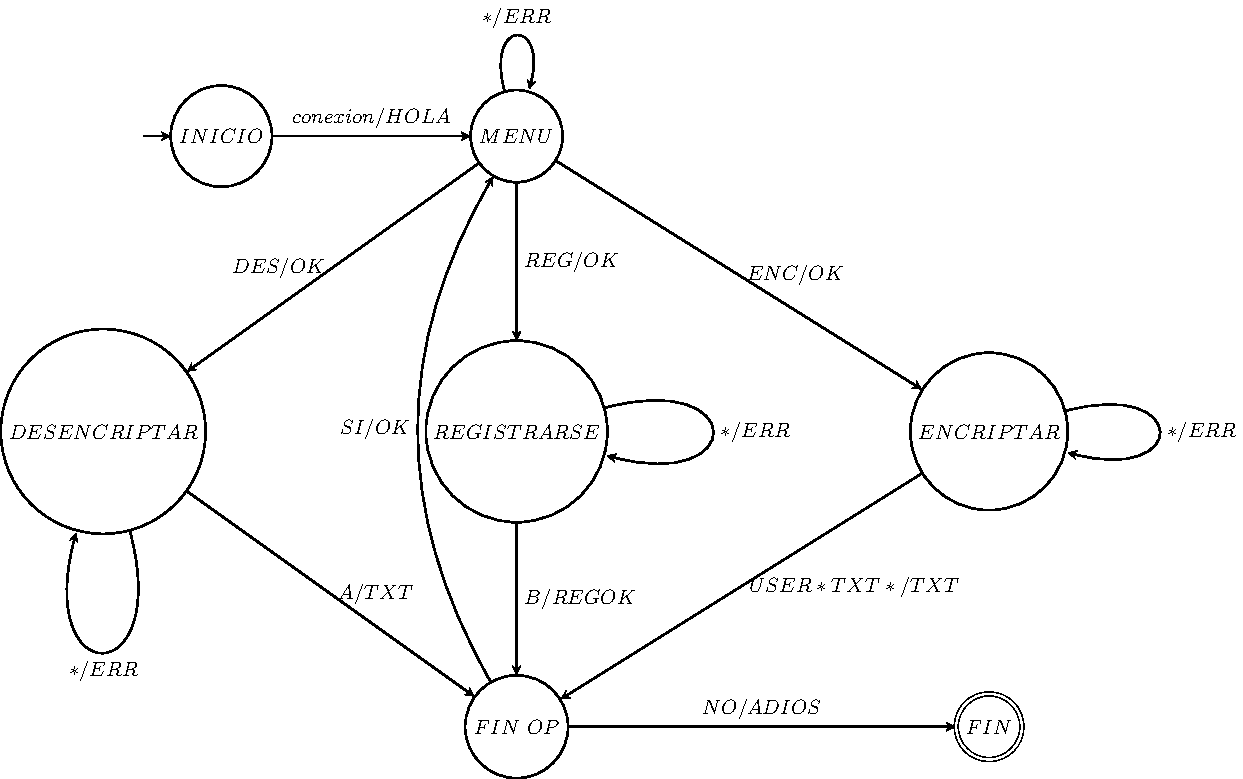
\includegraphics[width=15cm]{../pdf/diagrama.pdf}
	Donde $A=USER*PASS*TXT*$ \quad $B=USER*PASS*$ 
\newpage

\section{Mensajes que intervienen}

\begin{table}[h]
\centering
\begin{tabular}{|l|l|l|}
\hline
{Código} & {Cuerpo} & {Descripción}                        \\ \hline
1001                          & HOLA                          & Conexión establecida correctamente                        \\ \hline
1002                          & DES                           & Petición de desencriptacion                                     \\ \hline
1003                          & ENC                           & Petición de encriptación                                       \\ \hline
1004                          & REG                           & Petición de registro                                      \\ \hline
1005                          & OK                        	  & Opción escogida correcta                                      \\ \hline
1006                          & A                             & Mensaje con un texto a desencriptar y las\\  
							  & 							  & credenciales del receptor                                 \\ \hline
1007                          & TXT                           & Texto obtenido tras encriptar o \\
							  &                               &desencriptar \\ \hline
1008                          & B                         	  & Credenciales para registrarse                             \\ \hline
1009                          & REGOK                         & Registro exitoso                               \\ \hline
1010                          & $USER*TXT*$                   & Texto a encriptar y usario destino                            \\ \hline
1011                          & SI                            & Seguir realizando operaciones                                   \\ \hline
1012                          & ADIOS                         & Desconexión del programa                                  \\ \hline
\end{tabular}
\end{table}

\newpage
\section{Evaluaci\'on de la aplicaci\'on}

\end{document}
